% 第一部分：训练结果、最终策略的行为与代价（由 main_zh.tex 引入）。

\section{用评判模型的奖励训练}\label{sec:results}

全部 \NUM{runs_total} 个 run 都已完成：五个任务上的七种条件，每种 5 个种子（\texttt{ar\_sampled} 为 3 个）。虚拟机的一次重置中断了 \NUM{resumed_runs} 个 run（\NUM{resumed_conds}），它们从第 \NUM{resumed_steps} 步的检查点恢复，每个丢弃了当时进行中的回合，最多 \NUM{resumed_dropped_max} 步。表~\ref{tab:returns} 给出各任务的最终回报，表~\ref{tab:aggregate} 给出归一化后的汇总结果，图~\ref{fig:curves} 给出学习曲线。

\begin{table}[t]
\centering\footnotesize\setlength{\tabcolsep}{3pt}
\begin{tabular}{@{}lccccccc@{}}
\toprule
 task & \texttt{env} & \texttt{env\_window} & \texttt{kev\_score} & \texttt{kev\_gated} & \texttt{kev\_distill} & \texttt{ar\_gated} & \texttt{ar\_sampled} \\ \midrule
Hopper & 2820 $\pm$ 969 & 3419 $\pm$ 450 & 3061 $\pm$ 314 & 3169 $\pm$ 174 & 2833 $\pm$ 909 & 1165 $\pm$ 309 & 1127 $\pm$ 293 \\
Walker2d & 3150 $\pm$ 1276 & 4068 $\pm$ 1909 & 2593 $\pm$ 509 & 2536 $\pm$ 712 & 2943 $\pm$ 562 & 1321 $\pm$ 189 & 1330 $\pm$ 165 \\
HalfCheetah & 3441 $\pm$ 1152 & 2376 $\pm$ 1349 & 2845 $\pm$ 638 & 4241 $\pm$ 242 & 4117 $\pm$ 460 & 1069 $\pm$ 1046 & 1050 $\pm$ 824 \\
Swimmer & 81 $\pm$ 22 & 278 $\pm$ 104 & 99 $\pm$ 148 & 141 $\pm$ 124 & 91 $\pm$ 41 & 141 $\pm$ 120 & 118 $\pm$ 166 \\
Reacher & $-$6.4 $\pm$ 1.6 & $-$28.0 $\pm$ 9.4 & $-$48.9 $\pm$ 21.2 & $-$75.8 $\pm$ 10.9 & $-$88.4 $\pm$ 21.9 & $-$75.2 $\pm$ 21.3 & $-$68.8 $\pm$ 21.3 \\
\bottomrule
\end{tabular}

\caption{各任务的最终回报：训练 $10^6$ 步后，确定性策略在 20 个评估回合上的平均回报，再对种子取均值 $\pm$ 标准差。均匀随机策略的回报为 \NUM{rand_hopper}（Hopper）、\NUM{rand_walker}（Walker2d）、\NUM{rand_cheetah}（HalfCheetah）、\NUM{rand_swimmer}（Swimmer）和 \NUM{rand_reacher}（Reacher）。}
\label{tab:returns}
\end{table}

\begin{table}[t]
\centering\small
\begin{tabular}{@{}lcccccc@{}}
\toprule
condition & runs & IQM [95\% CI] & mean & median & $P(\,>\texttt{env})$ & $P(\,>\texttt{env\_window})$ \\ \midrule
\texttt{env} & 25 & 1.05 \ci{0.91}{1.16} & 1.00 & 1.03 & 0.50 & 0.46 \\
\texttt{env\_window} & 25 & 1.10 \ci{0.89}{1.26} & 1.41 & 1.21 & 0.54 & 0.50 \\
\texttt{kev\_score} & 25 & 0.78 \ci{0.60}{0.91} & 0.76 & 0.82 & 0.28 & 0.27 \\
\texttt{kev\_gated} & 25 & 1.00 \ci{0.81}{1.09} & 0.79 & 1.05 & 0.44 & 0.31 \\
\texttt{kev\_distill} & 25 & 0.98 \ci{0.82}{1.10} & 0.59 & 1.02 & 0.44 & 0.27 \\
\texttt{ar\_gated} & 25 & 0.35 \ci{0.28}{0.46} & 0.40 & 0.36 & 0.18 & 0.10 \\
\texttt{ar\_sampled} & 15 & 0.31 \ci{0.19}{0.45} & 0.37 & 0.36 & 0.12 & 0.11 \\
\bottomrule
\end{tabular}

\caption{全部任务和种子上的归一化分数 $(R-R_{\text{rand}})/(R_{\text{env}}-R_{\text{rand}})$：四分位均值（IQM）及其 95\% 分层 bootstrap 区间、均值、中位数，以及该条件的一个 run 在同一任务上胜过 \texttt{env} 或 \texttt{env\_window} 的一个 run 的概率（对任务取平均）。}
\label{tab:aggregate}
\end{table}

\begin{figure}[t]
\centering
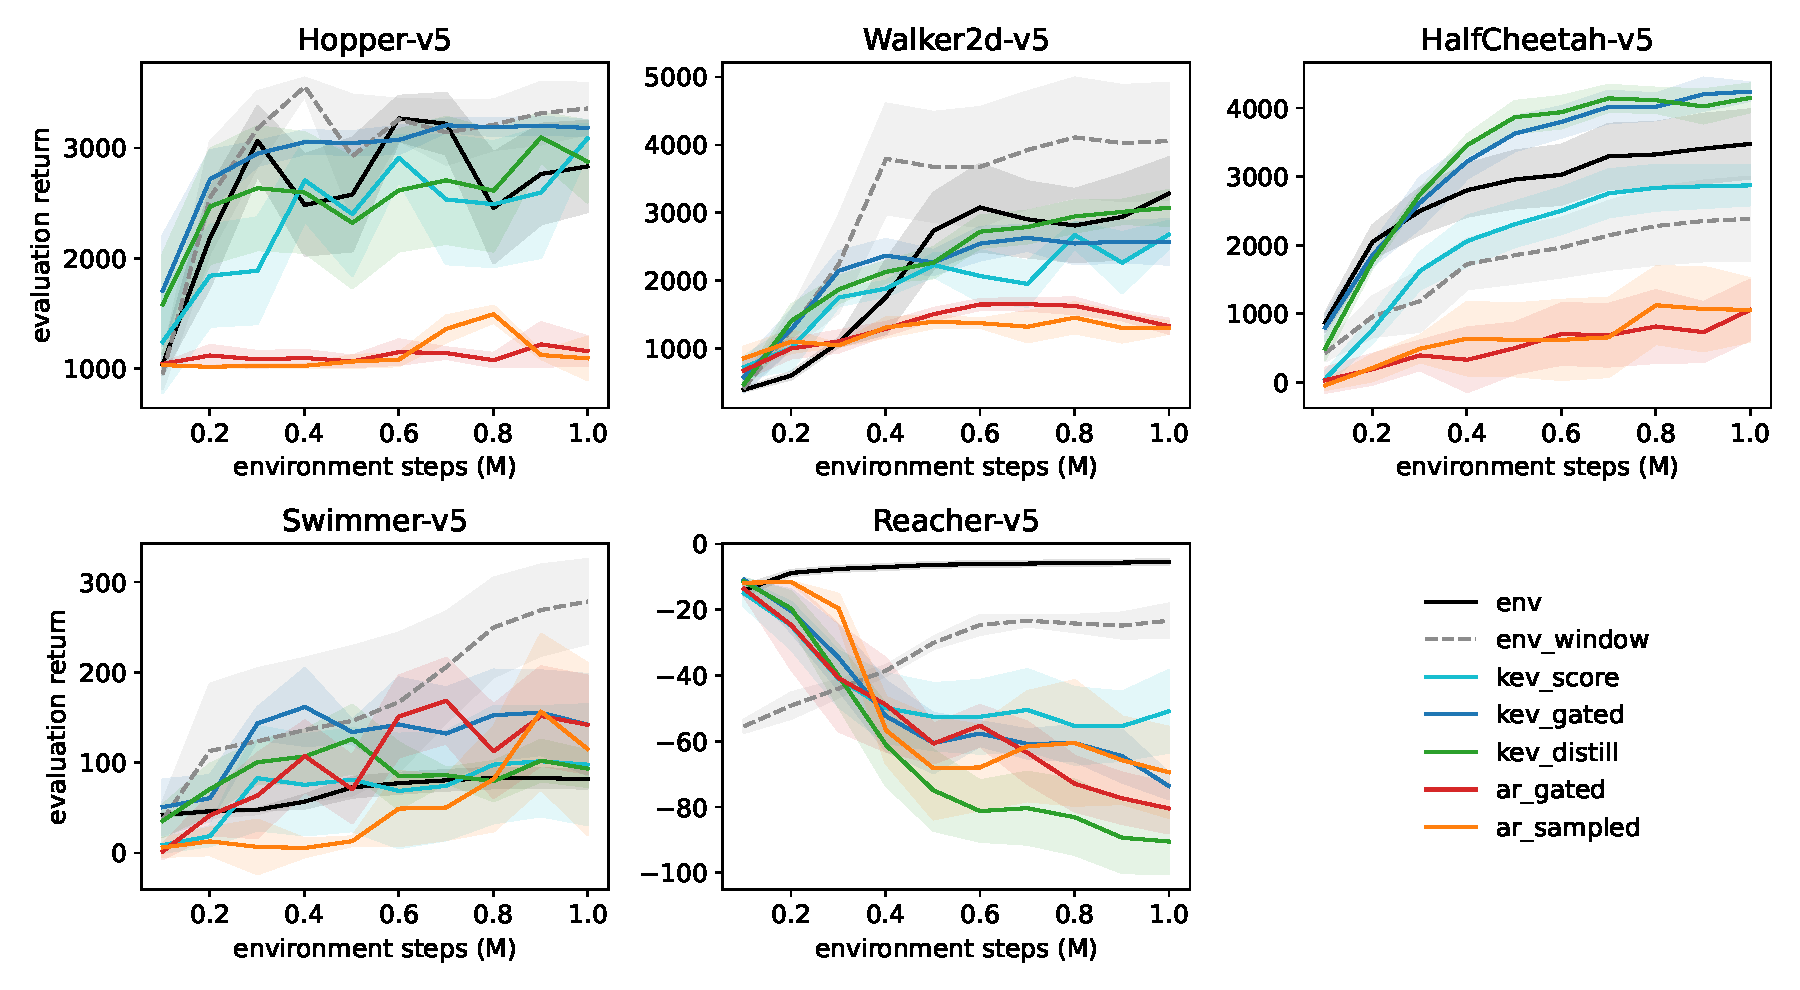
\includegraphics[width=\linewidth]{../../experiments/part1_control/results/learning_curves.pdf}
\caption{训练过程中的评估回报：每 $10^5$ 步评估 10 个回合，曲线为种子均值，阴影为 $\pm$ 一个标准误。}
\label{fig:curves}
\end{figure}

\paragraph{从汇总看，\kev{} 的门控奖励和蒸馏奖励接近工程化奖励，AR 评判的奖励则差得远。} 归一化分数的 IQM：\texttt{kev\_gated} 为 \NUM{iqm_kev_gated} \ci{\NUM{iqmlo_kev_gated}}{\NUM{iqmhi_kev_gated}}，\texttt{kev\_distill} 为 \NUM{iqm_kev_distill} \ci{\NUM{iqmlo_kev_distill}}{\NUM{iqmhi_kev_distill}}，\texttt{env} 为 \NUM{iqm_env} \ci{\NUM{iqmlo_env}}{\NUM{iqmhi_env}}，区间大幅重叠。在同一任务上，用这两种奖励训练的 run 胜过用工程化奖励训练的 run 的概率分别为 \NUM{pimpenv_kev_gated}（\texttt{kev\_gated}）和 \NUM{pimpenv_kev_distill}（\texttt{kev\_distill}）。去掉门控后，\kev{} 的分数表现更差（\NUM{iqm_kev_score} \ci{\NUM{iqmlo_kev_score}}{\NUM{iqmhi_kev_score}}，概率 \NUM{pimpenv_kev_score}）。AR 评判的奖励只达到工程化奖励归一化分数的三分之一左右：期望读出为 \NUM{iqm_ar_gated} \ci{\NUM{iqmlo_ar_gated}}{\NUM{iqmhi_ar_gated}}，采样读出为 \NUM{iqm_ar_sampled} \ci{\NUM{iqmlo_ar_sampled}}{\NUM{iqmhi_ar_sampled}}。在同一任务上，一个 \texttt{kev\_gated} run 胜过一个 \texttt{ar\_gated} run 的概率为 \NUM{pimp_all_kevgated_argated}；分任务看，Hopper 上为 \NUM{pimp_hopper_kevgated_argated}，HalfCheetah 上为 \NUM{pimp_cheetah_kevgated_argated}，Walker2d 上为 \NUM{pimp_walker_kevgated_argated}，而 Swimmer（\NUM{pimp_swimmer_kevgated_argated}）和 Reacher（\NUM{pimp_reacher_kevgated_argated}）上接近持平。

\paragraph{汇总掩盖了 Reacher。} IQM 去掉了最低和最高各四分之一的 run。均值更低：\texttt{kev\_gated} 为 \NUM{mean_kev_gated}，\texttt{kev\_distill} 为 \NUM{mean_kev_distill}。在 Reacher 上，每种评判奖励的最终结果都低于随机策略，因此这些 run 的归一化分数为负（表~\ref{tab:returns}）。所以我们逐个任务来看。

\paragraph{逐个任务。} 在 Hopper 上，\kev{} 的奖励最终接近工程化奖励（\texttt{kev\_gated} 为 \NUM{ret_hopper_kev_gated}，\texttt{env} 为 \NUM{ret_hopper_env}；改进概率 \NUM{pimp_hopper_kevgated_env}）。在 Walker2d 上它们更低（\texttt{kev\_gated} 为 \NUM{ret_walker_kev_gated}，\texttt{kev\_distill} 为 \NUM{ret_walker_kev_distill}，\texttt{env} 为 \NUM{ret_walker_env}；概率分别为 \NUM{pimp_walker_kevgated_env} 和 \NUM{pimp_walker_kevdistill_env}）。在 HalfCheetah 上，\texttt{kev\_gated}（\NUM{ret_cheetah_kev_gated}）和 \texttt{kev\_distill}（\NUM{ret_cheetah_kev_distill}）高于工程化奖励（\NUM{ret_cheetah_env}；两者的概率都是 \NUM{pimp_cheetah_kevgated_env}），原因见 \S\ref{sec:behaviour}。在 Swimmer 上，用工程化奖励训练的 PPO 几乎没让游动者动起来（\NUM{ret_swimmer_env}）；其他每种奖励的平均结果都更好，其中窗口平均的真实奖励最好（\NUM{ret_swimmer_env_window}），评判奖励在不同种子间差异很大。在 Reacher 上，只有工程化奖励学会了任务：用它为 \NUM{ret_reacher_env}，用它的窗口平均为 \NUM{ret_reacher_env_window}，用评判奖励为 \NUM{ret_reacher_kev_score} 到 \NUM{ret_reacher_kev_distill}。学习曲线显示，评判奖励训练的 Reacher 策略随着训练越来越差（图~\ref{fig:curves}）。

\paragraph{窗口级反馈在运动任务上代价很小，在 Reacher 上代价很大。} 在评判窗口上平均的真实奖励（\texttt{env\_window}）在汇总上至少不比逐步奖励差：IQM \NUM{iqm_env_window} \ci{\NUM{iqmlo_env_window}}{\NUM{iqmhi_env_window}}，改进概率 \NUM{pimpenv_env_window}。它在 Hopper（\NUM{pimp_hopper_envwindow_env}）、Walker2d（\NUM{pimp_walker_envwindow_env}）和 Swimmer（\NUM{pimp_swimmer_envwindow_env}）上领先；在 HalfCheetah 上落后（\NUM{pimp_cheetah_envwindow_env}），它的五个 run 中有 \NUM{flipruns_cheetah_env_window} 个最终翻成背朝下（\S\ref{sec:behaviour}）；在 Reacher 上也落后（\NUM{pimp_reacher_envwindow_env}）。一个 Reacher 回合只有两个 25 步的窗口，平均后的奖励不再告诉策略是哪些动作让指尖靠近了目标，其机械臂最终离目标并不比随机策略更近（表~\ref{tab:behaviour}）。因此，评判模型的时间分辨率能解释它们在 Reacher 上的部分失败，但完全解释不了 AR 评判在 Hopper 和 Walker2d 上的失败——在那里窗口平均奖励表现很好。

\paragraph{蒸馏只用十分之一的评判调用就保住了 \kev{} 的奖励。} \texttt{kev\_distill} 每个 run 只向评判模型询问 \NUM{judgewin_kev_distill} 个窗口，而不是 \NUM{judgewin_kev_gated} 个，最终与 \texttt{kev\_gated} 持平：IQM \NUM{iqm_kev_distill} 对 \NUM{iqm_kev_gated}，改进概率 \NUM{pimp_all_kevdistill_kevgated}。它最弱的任务是 Reacher（\NUM{ret_reacher_kev_distill}）。

\paragraph{训练中，两个评判模型的分数与奖励的相关程度相近。} 每个 run 对每次 rollout 记录了它所训练的窗口分数与同一批窗口的环境奖励之间的相关系数。对 rollout 和 run 取平均，\texttt{kev\_gated} 为 \NUM{traincorr_kev_gated}，\texttt{ar\_gated} 为 \NUM{traincorr_ar_gated}，而 \texttt{ar\_sampled} 只有 \NUM{traincorr_ar_sampled}——它的单次抽样大部分是噪声（\S\ref{sec:agreement}）。两种门控奖励与环境奖励的相关程度差不多，却训练出了截然不同的策略，下一节会说明这一点。

\subsection{策略学到了什么}\label{sec:behaviour}

回报并不说明策略做了什么。我们把每个最终策略在它的 20 个评估回合上重新运行一遍，记录机器人的实际行为（表~\ref{tab:behaviour}）。重新运行的回报与日志中的回报完全一致（最大差异 \NUM{beh_maxdiff}）。

\begin{table}[t]
\centering\small
\begin{tabular}{@{}lcccccc@{}}
\toprule
 & Hopper & Walker2d & Swimmer & HalfCheetah & \multicolumn{2}{c}{Reacher} \\ \cmidrule(lr){2-2}\cmidrule(lr){3-3}\cmidrule(lr){4-4}\cmidrule(lr){5-5}\cmidrule(l){6-7}
condition & still & still & still & runs flipped & effort & distance (m) \\ \midrule
\texttt{env} & 0\% & 1\% & 62\% & 1 of 5 & 0.01 & 0.101 \\
\texttt{env\_window} & 0\% & 0\% & 14\% & 3 of 5 & 0.19 & 0.180 \\
\texttt{kev\_score} & 0\% & 4\% & 11\% & 0 of 5 & 0.36 & 0.256 \\
\texttt{kev\_gated} & 1\% & 10\% & 15\% & 0 of 5 & 0.63 & 0.263 \\
\texttt{kev\_distill} & 1\% & 1\% & 11\% & 0 of 5 & 0.76 & 0.250 \\
\texttt{ar\_gated} & 49\% & 40\% & 18\% & 0 of 5 & 0.63 & 0.253 \\
\texttt{ar\_sampled} & 26\% & 17\% & 50\% & 0 of 3 & 0.56 & 0.252 \\ \midrule
random policy & 31\% & 4\% & 26\% & -- & 0.33 & 0.180 \\
\bottomrule
\end{tabular}

\caption{最终策略的行为，对回合和种子取平均（每个 run 20 个评估回合）。\emph{still}：$|v_x|<0.1$\,m/s 的步数占比。\emph{runs flipped}：猎豹有一半以上步数背朝下（$\cos(\text{pitch})<0$）的 run 数。\emph{effort}：动作平方的均值，取值于 $[0,1]$。\emph{distance}：一个回合中指尖到目标的平均距离。随机策略从均匀分布中采样动作。}
\label{tab:behaviour}
\end{table}

\begin{table}[t]
\centering\small
\begin{tabular}{@{}lcccccc@{}}
\toprule
 & & & \multicolumn{2}{c}{\kev{}} & \multicolumn{2}{c}{AR judge} \\ \cmidrule(lr){4-5}\cmidrule(l){6-7}
task & windows (slow / fast) & env.\ reward & progress & gated & progress & gated \\ \midrule
Hopper & 42 / 430 & 0.31 & 0.59 & 0.48 & 0.89 & 0.87 \\
Walker2d & 386 / 1238 & 0.27 & 0.62 & 0.47 & 0.90 & 0.87 \\
HalfCheetah & 309 / 1368 & $-$0.06 & 0.51 & 0.15 & 0.85 & 0.65 \\
\bottomrule
\end{tabular}

\caption{在 \S\ref{sec:agreement} 的窗口（\texttt{env} 条件的 run 记录的窗口）上，每种信号给“站着”相对于“跑”的报酬。表中数值为：未摔倒且慢于 \NUM{sf_slowmax}\,m/s 的窗口上的均值，除以快于 \NUM{sf_fastmin}\,m/s 的窗口上的均值。\emph{env.\ reward}：逐步环境奖励。}
\label{tab:slowfast}
\end{table}

\paragraph{AR 评判的奖励让单腿跳跃机器人和双足行走机器人学会了站着。} 最终的 \texttt{ar\_gated} 策略在 Hopper 上有 \NUM{still_hopper_ar_gated} 的步数站着不动，在 Walker2d 上为 \NUM{still_walker_ar_gated}。\texttt{kev\_gated} 的对应数字是 \NUM{still_hopper_kev_gated} 和 \NUM{still_walker_kev_gated}，\texttt{env} 为 \NUM{still_hopper_env} 和 \NUM{still_walker_env}。它们的平均前进速度为 \NUM{vx_hopper_ar_gated} 和 \NUM{vx_walker_ar_gated}\,m/s，而 \texttt{kev\_gated} 为 \NUM{vx_hopper_kev_gated} 和 \NUM{vx_walker_kev_gated}\,m/s，\texttt{env} 为 \NUM{vx_hopper_env} 和 \NUM{vx_walker_env}\,m/s。它们在 Hopper 上的回报（\NUM{ret_hopper_ar_gated}）接近 1000，也就是在一个 1000 步的回合里一直站着、仅靠存活奖励就能拿到的分数。对等级采样并不能消除这一现象：\texttt{ar\_sampled} 在两个任务上站着不动的步数占比为 \NUM{still_hopper_ar_sampled} 和 \NUM{still_walker_ar_sampled}。

表~\ref{tab:slowfast} 说明了原因。它比较每种信号给一个慢于 \NUM{sf_slowmax}\,m/s 的直立窗口和一个快于 \NUM{sf_fastmin}\,m/s 的窗口各付多少。AR 评判的门控分数在 Hopper 上给慢窗口的报酬是快窗口的 \NUM{sfratio_hopper_argated}（\NUM{sfs_hopper_argated} 对 \NUM{sff_hopper_argated}），在 Walker2d 上是 \NUM{sfratio_walker_argated}。工程化奖励只付 \NUM{sfratio_hopper_perstep} 和 \NUM{sfratio_walker_perstep}，\kev{} 的门控分数付 \NUM{sfratio_hopper_kevgated} 和 \NUM{sfratio_walker_kevgated}。回合中的每一步都得到其所在窗口的分数，而摔倒会结束回合。因此在 AR 评判的奖励下，直立站着每一步挣得几乎和跳跃一样多，又没有摔倒的风险。PPO 很早就找到了这一点：Hopper 上 \texttt{ar\_gated} 的曲线从第一次评估起就是平的（图~\ref{fig:curves}）。然而 AR 评判的分数对窗口的排序几乎和 \kev{} 一样好：它们与奖励的 Spearman 相关系数在 Hopper 上为 \NUM{rho_hopper_ar_gated} 对 \NUM{rho_hopper_kev_gated}，在 Walker2d 上为 \NUM{rho_walker_ar_gated} 对 \NUM{rho_walker_kev_gated}（表~\ref{tab:agreement}）。不同的是差距：AR 评判几乎把每个直立窗口都打在其分数范围的顶端。与奖励的排序一致性并没有预示出 PPO 能用上哪种奖励。

\paragraph{评判模型的奖励让猎豹保持直立。} 在 HalfCheetah 上，\texttt{env} 的五个 run 中有 \NUM{flipruns_cheetah_env} 个、\texttt{env\_window} 的五个 run 中有 \NUM{flipruns_cheetah_env_window} 个最终让猎豹背朝下。这是一个工程化奖励不加惩罚的局部最优。这些 run 的回报最多为 \NUM{flip_maxret}，而同样两种条件下保持直立的 run 至少为 \NUM{upright_minret}。用评判奖励训练的 \NUM{judge_runs_cheetah} 个 run 中没有一个翻倒。两个评判模型读到的任务描述都写明翻倒是不希望出现的，最低的 \texttt{progress} 等级也点了它的名。去掉翻倒的那个 run 后，\texttt{env} 在 HalfCheetah 上的平均回报为 \NUM{uprightret_env}，\texttt{kev\_gated} 为 \NUM{ret_cheetah_kev_gated}，所以 \kev{} 在这里的优势很大一部分来自翻倒。在这个例子里，评判模型的奖励带有工程化奖励所缺少的偏好，而策略遵循了它。

\paragraph{在 Reacher 上，评判模型的奖励让机械臂乱甩。} 用评判奖励训练的机械臂，指尖离目标的平均距离为 \NUM{dist_reacher_kev_distill} 到 \NUM{dist_reacher_kev_gated}\,m，比随机策略（\NUM{dist_reacher_random}\,m）和工程化奖励（\NUM{dist_reacher_env}\,m）都远。它们的控制力度也高于随机策略：\NUM{effort_reacher_kev_score} 到 \NUM{effort_reacher_kev_distill}，随机策略为 \NUM{effort_reacher_random}，\texttt{env} 为 \NUM{effort_reacher_env}。Reacher 的奖励每一步都按动作的平方扣分，这就是这些策略最终低于随机策略的原因。两个评判模型的分数跟随的是窗口内距离的变化（\kev{} 与 AR 评判的 \texttt{progress} 的 Spearman 相关系数分别为 \NUM{rhophys_reacher_kev_progress} 和 \NUM{rhophys_reacher_ar_progress}，\S\ref{sec:agreement}），而对 Reacher 奖励每一步都在计算的距离本身跟随得少得多（与奖励的相关系数为 \NUM{rho_reacher_kev_progress} 和 \NUM{rho_reacher_ar_progress}）。每个回合只有两个窗口，这两种信号都没能把 PPO 引到目标上。

\section{代价}\label{sec:cost}

\begin{table}[t]
\centering\small
\begin{tabular}{@{}lcccc@{}}
\toprule
condition & judged windows & judge wait (h) & wall-clock (h) & corr.\ (score, env reward) \\ \midrule
\texttt{env} & 0 & 0.0 & 0.1 & -- \\
\texttt{env\_window} & 0 & 0.0 & 0.1 & -- \\
\texttt{kev\_score} & 33{,}914 & 2.0 & 2.1 & 0.57 \\
\texttt{kev\_gated} & 33{,}942 & 1.9 & 2.1 & 0.56 \\
\texttt{kev\_distill} & 3{,}477 & 1.9 & 2.0 & 0.54 \\
\texttt{ar\_gated} & 33{,}861 & 1.9 & 2.0 & 0.52 \\
\texttt{ar\_sampled} & 33{,}869 & 1.9 & 2.0 & 0.17 \\
\bottomrule
\end{tabular}

\caption{每个 run 的代价，对任务和种子取平均：发送给评判模型的窗口数、等待其回答的时间、run 的总耗时，以及每次 rollout 中 run 所训练的窗口分数与同一批窗口的环境奖励之间相关系数的均值。一个 GPU 上的一个评判服务器同时服务最多 24 个 run，因此等待时间包含了它处理其他 run 请求的时间。}
\label{tab:cost}
\end{table}

表~\ref{tab:cost} 给出评判模型在每个 run 上的代价。对每个窗口都询问评判模型的 run，在 $10^6$ 步中大约发送 \NUM{judgewin_kev_gated} 个窗口，\texttt{kev\_distill} 大约发送 \NUM{judgewin_kev_distill} 个。不用评判模型的 run 耗时 \NUM{wallh_env}\,h；用评判模型的 run 耗时约 \NUM{wallh_kev_gated}\,h，约为前者的 \NUM{wallratio} 倍，其中几乎全部（\NUM{waith_kev_gated}\,h）花在等待评判上。这些时间反映的是我们的设置：一个 GPU 上的一个评判服务器同时回答最多 24 个 run 的请求，一个 run 的等待时间包含了服务器处理其他 run 请求的时间。这也是为什么 \texttt{kev\_distill} 只有十分之一的窗口，等待时间却差不多（\NUM{waith_kev_distill}\,h）：它的请求排在其他 run 的请求后面。我们没有测量评判模型只服务一个 run 的情形，而蒸馏奖励的节省会在那种情形下体现出来。
